\documentclass[border=4pt]{standalone}
\usepackage{amsmath,amssymb}
\usepackage{tikz}
\usetikzlibrary{arrows.meta,decorations.pathreplacing,patterns,calc,positioning,shapes.geometric}
\usepackage{pgfplots}
\pgfplotsset{compat=newest}
\begin{document}
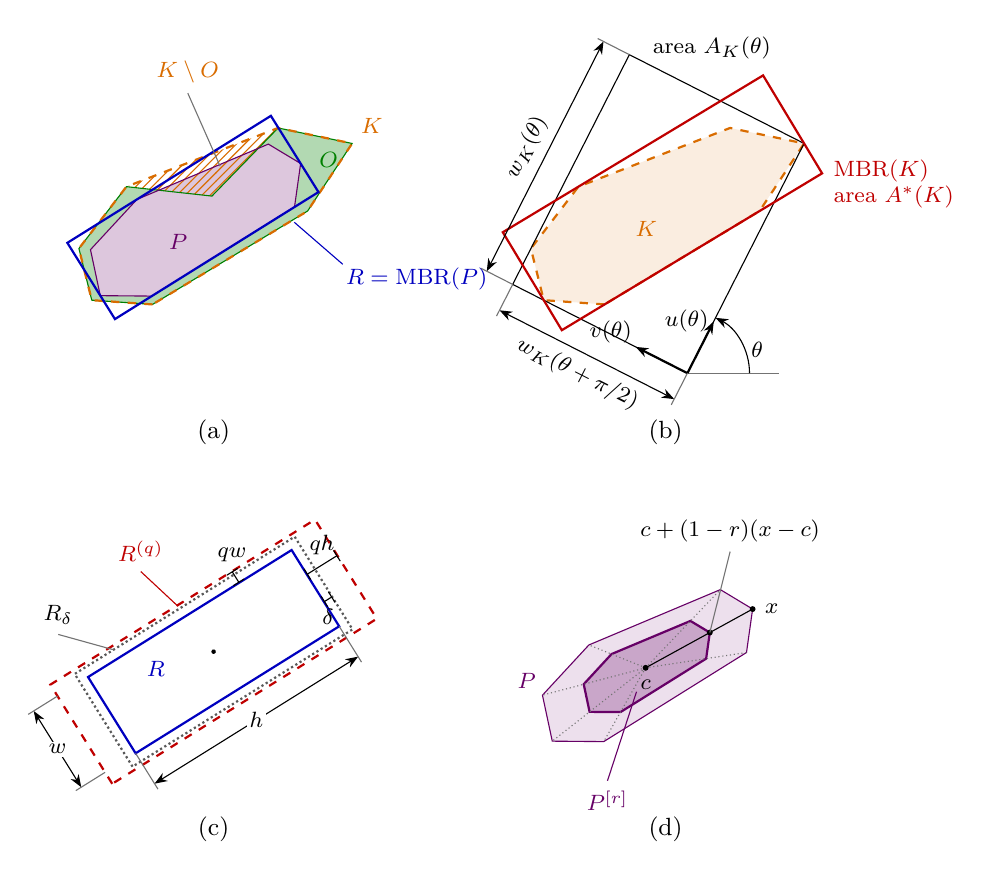
\begin{tikzpicture}[scale=0.82,
  >={Stealth[length=1.6mm]},
  lab/.style={font=\footnotesize},
  dim/.style={<->,thin},
  ext/.style={thin,black!55}]
\colorlet{colO}{green!50!black}
\colorlet{colK}{orange!85!black}
\colorlet{colP}{violet!80!black}
\colorlet{colR}{blue!75!black}
\def\Opath{(-1.887,-1.456) -- (-0.946,-1.522) -- (1.456,-0.075) -- (2.145,0.971) -- (0.999,1.211) -- (-0.026,0.156) -- (-1.350,0.302) -- (-2.086,-0.656) -- cycle}
\def\Kpath{(-0.946,-1.522) -- (-1.887,-1.456) -- (-2.086,-0.656) -- (-1.350,0.302) -- (0.999,1.211) -- (2.145,0.971) -- (1.456,-0.075) -- cycle}
\def\Ppath{(-1.755,-1.386) -- (-0.958,-1.393) -- (1.253,-0.013) -- (1.348,0.660) -- (0.848,0.961) -- (-1.188,0.104) -- (-1.907,-0.674) -- cycle}
%======================== (a) instance, hull, proposal, proposal rectangle
\begin{scope}
  \fill[colO!30] \Opath;
  \fill[colP!22] \Ppath;
  \fill[pattern=north east lines,pattern color=colK,even odd rule] \Kpath \Opath;
  \draw[colO] \Opath;
  \draw[colK,thick,dashed] \Kpath;
  \draw[colP] \Ppath;
  \draw[colR,thick] (-1.528,-1.749) -- (1.624,0.218) -- (0.887,1.399) -- (-2.265,-0.568) -- cycle;
  \node[lab,colO] at (1.78,0.72) {$O$};
  \draw[ext] (0.1,0.62) -- (-0.4,1.75) node[lab,colK,anchor=south] {$K\setminus O$};
  \node[lab,colK] at (2.45,1.25) {$K$};
  \node[lab,colP] at (-0.55,-0.55) {$P$};
  \draw[ext,colR] (1.25,-0.25) -- (2.0,-0.9) node[lab,anchor=north west,inner sep=1pt] {$R=\mathrm{MBR}(P)$};
  \node[font=\small] at (0,-3.5) {(a)};
\end{scope}
%======================== (b) widths, oriented rectangle and minimum-area rectangle of K
\begin{scope}[xshift=7.0cm]
  \fill[colK!12] \Kpath;
  \draw[colK,thick,dashed] \Kpath;
  % rectangle with sides parallel to u(theta), v(theta), theta = 63.1 deg
  \draw[thin] (0.338,-2.587) -- (2.145,0.971) -- (-0.561,2.346) -- (-2.368,-1.212) -- cycle;
  % minimum-area rectangle of K
  \draw[red!75!black,thick] (-1.607,-1.921) -- (2.424,0.508) -- (1.510,2.025) -- (-2.521,-0.404) -- cycle;
  % frame and angle at the corner (0.338,-2.587)
  \draw[ext] (0.338,-2.587) -- (1.75,-2.587);
  \draw[->,thick] (0.338,-2.587) -- ++(0.408,0.802) node[lab,anchor=east,inner sep=1.5pt] {$u(\theta)$};
  \draw[->,thick] (0.338,-2.587) -- ++(-0.802,0.408) node[lab,anchor=south east,inner sep=1pt] {$v(\theta)$};
  \draw[->,thin] (1.30,-2.587) arc[start angle=0,end angle=63.07,radius=0.962];
  \node[lab] at (1.42,-2.22) {$\theta$};
  % width in direction theta, along the side parallel to u(theta)
  \draw[dim] ($(-2.368,-1.212)+(-0.401,0.204)$) -- node[lab,sloped,above] {$w_K(\theta)$} ($(-0.561,2.346)+(-0.401,0.204)$);
  \draw[ext] (-2.368,-1.212) -- ++(-0.49,0.25);
  \draw[ext] (-0.561,2.346) -- ++(-0.49,0.25);
  % width in direction theta + pi/2, along the side parallel to v(theta)
  \draw[dim] ($(-2.368,-1.212)+(-0.204,-0.401)$) -- node[lab,sloped,below] {$w_K(\theta+\pi/2)$} ($(0.338,-2.587)+(-0.204,-0.401)$);
  \draw[ext] (-2.368,-1.212) -- ++(-0.25,-0.49);
  \draw[ext] (0.338,-2.587) -- ++(-0.25,-0.49);
  \node[lab,anchor=west] at (-0.35,2.45) {area $A_K(\theta)$};
  \node[lab,red!75!black,anchor=west] at (2.45,0.55) {$\mathrm{MBR}(K)$};
  \node[lab,red!75!black,anchor=west] at (2.45,0.15) {area $A^*(K)$};
  \node[lab,colK] at (-0.3,-0.35) {$K$};
  \node[font=\small] at (0,-3.5) {(b)};
\end{scope}
%======================== (c) rectangle operations, in the frame of R (long side horizontal)
\begin{scope}[yshift=-6.9cm]
\begin{scope}[rotate=31.96]
  % R: long side h = 3.715, short side w = 1.392; delta = 0.15, q = 0.15
  \draw[black!65,densely dotted,thick] (-2.008,-0.846) rectangle (2.008,0.846);
  \draw[red!75!black,dashed,thick] (-2.415,-0.905) rectangle (2.415,0.905);
  \draw[colR,thick] (-1.858,-0.696) rectangle (1.858,0.696);
  \fill (0,0) circle (1pt);
  % side lengths of R
  \draw[dim] (-1.858,-1.25) -- node[lab,fill=white,inner sep=1pt] {$h$} (1.858,-1.25);
  \draw[ext] (-1.858,-0.696) -- (-1.858,-1.35); \draw[ext] (1.858,-0.696) -- (1.858,-1.35);
  \draw[dim] (-2.85,-0.696) -- node[lab,fill=white,inner sep=1pt] {$w$} (-2.85,0.696);
  \draw[ext] (-2.415,-0.696) -- (-2.95,-0.696); \draw[ext] (-2.415,0.696) -- (-2.95,0.696);
  % margins: delta for R_delta, qw and qh for R^(q)
  \draw[|-|,thin] (1.858,0.25) -- node[lab,above] {$qh$} (2.415,0.25);
  \draw[|-|,thin] (1.858,-0.25) -- node[lab,below] {$\delta$} (2.008,-0.25);
  \draw[|-|,thin] (0.9,0.696) -- (0.9,0.905) node[lab,anchor=south] {$qw$};
  \node[lab,colR] at (-0.9,0.25) {$R$};
  \draw[ext] (-1.3,0.846) -- (-1.9,1.5) node[lab,black,anchor=south] {$R_\delta$};
  \draw[ext,red!75!black] (-0.1,0.905) -- (-0.3,1.65) node[lab,anchor=south] {$R^{(q)}$};
\end{scope}
  \node[font=\small] at (0,-2.75) {(c)};
\end{scope}
%======================== (d) homothetic contraction of P about its centroid
\begin{scope}[xshift=7.0cm,yshift=-6.9cm]
  \def\Prpath{(-1.177,-0.932) -- (-0.699,-0.936) -- (0.628,-0.108) -- (0.685,0.296) -- (0.385,0.476) -- (-0.837,-0.037) -- (-1.268,-0.504) -- cycle}
  \fill[colP!12] \Ppath;
  \draw[colP] \Ppath;
  \fill[colP!35] \Prpath;
  \draw[colP,thick] \Prpath;
  \foreach \v in {(-1.755,-1.386),(-0.958,-1.393),(1.253,-0.013),(0.848,0.961),(-1.188,0.104),(-1.907,-0.674)}
    \draw[ext,densely dotted] (-0.309,-0.250) -- \v;
  \draw[thin] (-0.309,-0.250) -- (1.348,0.660);
  \fill (-0.309,-0.250) circle (1.3pt) node[lab,below=1pt] {$c$};
  \fill (1.348,0.660) circle (1.3pt) node[lab,right=1pt] {$x$};
  \fill (0.685,0.296) circle (1.3pt);
  \draw[ext] (0.685,0.296) -- (1.0,1.55) node[lab,black,anchor=south] {$c+(1-r)(x-c)$};
  \node[lab,colP] at (-2.15,-0.45) {$P$};
  \draw[ext,colP] (-0.45,-0.62) -- (-0.9,-2.0) node[lab,anchor=north] {$P^{[r]}$};
  \node[font=\small] at (0,-2.75) {(d)};
\end{scope}
\end{tikzpicture}
\end{document}
